%!TEX root = ../rapport.tex
%!TEX encoding = UTF-8 Unicode

% Chapitres "Introduction"

% modifié par Francis Valois, Université Laval
% 31/01/2011 - version 1.0 - Création du document

\chapter{Description des cas d'utilisation}
\label{s:utilisation}
Cette section contient un résumé de chacun des différents cas d'utilisation. Elle est divisée en trois sous-sections: soit les cas d'utilisation en lien à l'usager, ceux en lien à la station de base et finalement ceux en lien au robot. Le diagramme des cas d'utilisation est présenté à la section \ref{use_cases}.
\section{Cas d'utilisation en lien avec l'usager}
\subsection{Lancer le signal de départ}
À l'aide d'un Graphical user interface ou interface graphique pour utilisateur (GUI) installé sur la station de base, l'utilisateur clique sur un bouton qui permet au robot de lancer son exécution (signal de départ transmis au robot pour commencer à effectuer une tâche).
\subsection{Entrer les coordonnées initiales du robot}
Avant d'envoyer le signal de départ au robot, l'utilisateur doit pouvoir entrer dans le GUI de la station de base les coordonnées de la position de départ du robot par rapport au terrain de jeu.
\section{Cas d'utilisations en lien avec la station de base}
\subsection{Localiser le robot}
À l'aide de la Kinect, la station de base doit être en mesure de trouver la position du robot sur le terrain de jeu.
\subsection{Détecter les obstacles}
La station de base, au moyen de la Kinect, doit pouvoir à détecter la position des deux obstacles disposés entre les deux zones principales du terrain de jeu, ainsi que les limites (murs) du terrain.
\subsection{Afficher la solution du sudocube}
La station de base doit être capable d'afficher une image du sudocube résolu et d'indiquer à l'écran le chiffre qui se trouve dans la case rouge du sudocube.
\subsection{Afficher le message de confirmation du lancement de la tâche}
La station doit être capable d'afficher un message de confirmation du lancement de la tâche pour l'usager lorsque le message de confirmation du robot est reçu.
\subsection{Afficher la trajectoire prévue et réelle du robot}
La trajectoire calculée et transmise par le robot doit être affichée à l'écran de la station de base. De plus, à l'aide des données fréquemment transmises par la Kinect contenant la position du robot, la station doit afficher, en comparaison à la trajectoire prévue, la trajectoire réelle du robot.
\subsection{Transmettre des données au robot}
La station doit transmettre au robot, par connexion sans fil, des messages indiquant de lancer une nouvelle tâche, la position des obstacles et la position de ces derniers.
\subsection{Recevoir des données provenant du robot}
La station de base doit être capable de recevoir, par connexion sans fil, des données provenant du robot comme la trajectoire que le robot prévoit emprunter, le sudocube résolu, le message de confirmation du lancement d'une tâche et le message indiquant la fin d'une tâche.
\subsection{Afficher le message confirmant que la tâche a été complétée avec succès ou a échoué}
La station de base doit afficher un message à l'écran confirmant que la tâche a été complétée avec succès ou un message d'échec si cette dernière a pris de plus de 10 minutes pour s'exécuter.
\subsection{Afficher le temps d'exécution de la tâche}
La station de base doit être en mesure d'afficher à l'écran le temps d'exécution de la tâche.
\section{Cas d'utilisation en lien avec le robot}
\subsection{Déterminer le chemin optimal entre un point A et un point B tout en évitant les obstacles}
En connaissant la configuration et la position des obstacles, le robot doit calculer la trajectoire optimale qu'il doit emprunter pour se rendre d'un point à un autre.
\subsection{Se déplacer d'un point A au point B}
Le robot doit être capable de se déplacer, sur le terrain de jeu, d'un point A vers un point B avec un contrôle automatisé des roues.
\subsection{Indiquer son adresse IP locale pour que la station de base puisse communiquer avec le robot}
Le robot doit être capable d'indiquer son adresse IP locale à la station de base pour que celle-ci établisse une connexion sans fil avec le robot.
\subsection{Extraire les informations d'un sudocube à partir d'une photo}
À l'aide d'une caméra embarquée sur le robot, il doit prendre une photo et représenter le sudocube à partir de l'image obtenue.
\subsection{Résoudre le sudocube et identifier le chiffre dans le carré rouge}
Le robot doit effectuer des traitements sur l'image du sudocube afin de le représenter et de le résoudre par la suite. Il identifie également l'emplacement de la case rouge à l'intérieur du sudocube et détermine donc le chiffre qui s'y trouve.
\subsection{Recevoir des données provenant de la station de base}
Le robot doit être capable de recevoir, par connexion sans fil avec la station de base, des messages indiquant de lancer une nouvelle tâche, la position des obstacles et sa position.
\subsection{Transmettre des données à la station de base}
Le robot doit transmettre, par connexion sans-fil, des données à la station de base comme la trajectoire que le robot prévoit emprunter, le sudocube résolu, le message de confirmation du lancement d'une tâche et le message indiquant la fin d'une tâche.
\subsection{Contrôler une DEL}
Une fois le message de fin de tâche transmis et le robot à l'extérieur de l'air de dessin, ce dernier doit allumer une DEL qui est installée sur le robot.
\subsection{Lancer de nouvelles tâches si la compétition n'est pas terminée}
Si le temps alloué pour la compétition (10 minutes) n'est pas écoulé, le robot doit commencer une nouvelle tâche après en avoir terminer la séquence d'opération.
\subsection{Se localiser}
Le robot doit être capablee en tout temps de déterminer sa position et son orientation, à l'aide de la webcam et des données reçues, ce qu'il lui permet de connaître son emplacement par rapport à l'antenne, aux murs, aux obstacles et aux sudocubes. De plus, il doit transmettre ces données à la station de base de façon régulière.
\subsection{Décoder la transmission de l'antenne}
Le robot doit se déplacer au-dessus de l'antenne et de capter le signal transmis par celle-ci. Il doit ensuite le décoder pour trouver les paramètres indiquant le sudocube ciblé ainsi que l'orientation et la taille du chiffre à dessiner dans la zone de base.
\subsection{Dessiner, en suivant les consignes, le chiffre prélevé dans le carré rouge}
Le robot doit utiliser un préhenseur afin de poser la mine du crayon sur la table, une fois dans l'air de dessin. Il doit ensuite se déplacer de façon à dessiner le chiffre trouvé dans la case rouge du sudocube, tout en suivant les dimensions exigées et les paramètres décodés. 
\subsection{Afficher des informations sur l'écran LCD}
Les paramètres trouvés lors du décodage du signal de l'antenne doivent être affichés sur un écran LCD installé sur le robot.
\section{Diagramme des cas d'utilisation}
\label{use_cases}
\addtolength{\evensidemargin}{-1in}	
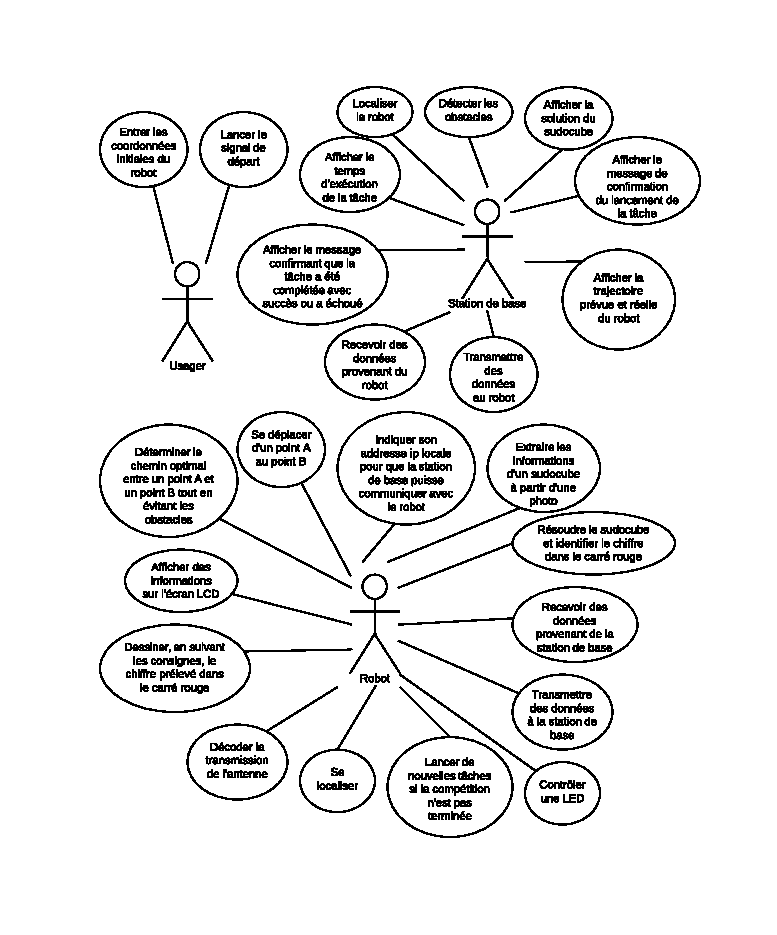
\includepdf[scale= 1]{use_cases_diagram.pdf}